\subsection{Leibniz on Integration: The General Area of a Curve}  

While differentiation described instantaneous motion, both Newton and Leibniz recognized that integration was its inverse which allowed them to compute the area under a curve.  

Newton thought of integration as summing up infinitesimally small changes in position (essentially reconstructing motion from its velocity).  

Leibniz, on the other hand, created the notation we still use today:

\[
\int dy
\]

But unlike Kepler, who used area to study planetary motion, Newton and Leibniz’s methods could describe any curve, anywhere, in any context (i.e. a falling cannonball, a planet, or even a changing economic trend).  

\begin{figure}[H]
\centering
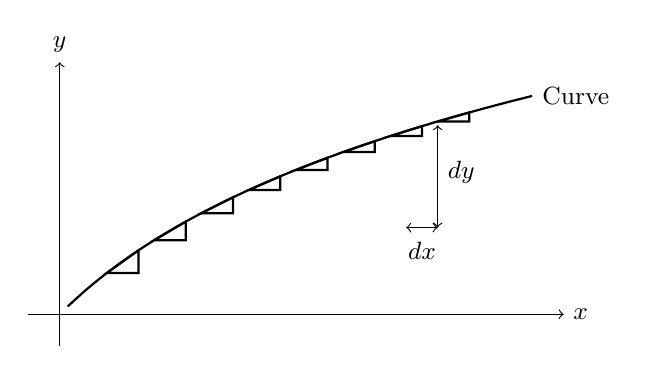
\begin{tikzpicture}[scale=2]
    % Axes
    \draw[->] (-0.2, 0) -- (3.2, 0) node[right] {\small $x$};
    \draw[->] (0, -0.2) -- (0, 1.6) node[above] {\small $y$};

    % Curve (logarithmic function)
    \draw[thick, domain=0.05:3, smooth, variable=\x] plot ({\x},{ln(\x + 1)}) node[right] {\small Curve};

    % Infinitesimal rectangles along the curve
    \foreach \x in {0.3, 0.6, 0.9, 1.2, 1.5, 1.8, 2.1, 2.4} {
        \draw[thick] (\x, {ln(\x + 1)}) -- ({\x + 0.2}, {ln(\x + 1)}) -- ({\x + 0.2}, {ln(\x + 1.2)}) -- cycle;
    }

    % Labels for differentials
    \node at (2.3, 0.4) {\small $dx$};
    \node at (2.55, 0.9) {\small $dy$}; % moved down

    % Arrows showing differential elements
    \draw[<->] (2.2, 0.55) -- (2.4, 0.55);
    \draw[<->] (2.4, 0.55) -- (2.4, 1.2);
\end{tikzpicture}

\vspace{0.5em}
\caption{\small A logarithmic curve with infinitesimal rectangles illustrating the differentials $dx$ and $dy$. The horizontal arrow represents a small fixed change in $x$, while the vertical arrow shows the actual change in $y$ over that interval: $dy = \ln(x+dx+1) - \ln(x+1)$. Since the slope of the function increases with $x$, $dy$ becomes larger for the same $dx$. This reflects the local steepness of the curve and highlights the geometric meaning of the derivative as the ratio $\frac{dy}{dx}$.}
\end{figure}


In Leibniz’s framework, a curve was analyzed through the use of differentials. At any point along the curve, one could consider an infinitesimal triangle formed by two small changes: the horizontal difference, denoted by $dx$, and the corresponding vertical difference, denoted by $dy$. These represented the vanishingly small increments of the variable and its ordinate. The slope of the curve at that point was expressed by the ratio $\frac{dy}{dx}$, which Leibniz interpreted as the differential quotient — the rate at which one quantity changed with respect to another. Though Leibniz focused primarily on these differential relationships, the infinitesimal triangles hinted at a broader method: by summing such differentials along the curve, one could conceive of a total quantity accumulated — an idea that would later be formalized as the integral.

\subsubsection{Leibniz’s View: Infinitesimals, Not Triangles}

Where Newton envisioned geometry in motion, Leibniz saw motion in algebra.

Galileo had shown that a falling body accelerates uniformly — covering distance in proportion to the square of time. But this, for Leibniz, was not merely a fact of nature; it was a structure waiting for notation. He took Galileo’s parabolas and velocities and rewrote them as relations between differentials.


\subsubsection{A New Language of Change} 

Leibniz conceived of motion as a relation between infinitely small changes. If $s$ is the vertical distance fallen and $t$ is time, then:

\[
\frac{ds}{dt} = v(t)
\]

\begin{figure}[H]
  \centering
  \begin{tikzpicture}[scale=1.2]
  
    % Axes
    \draw[->] (0,0) -- (5.5,0) node[right] {$t$ (tempus)};
    \draw[->] (0,0) -- (0,3.5) node[above] {$s$ (spatium)};
  
    % Position curve: s(t) = ln(t + 1)
    \draw[thick,blue,domain=0:5,smooth,samples=100] plot(\x,{1.5*ln(\x + 1)});
    \node[blue] at (4.2,2.8) {\footnotesize $s(t) = \ln(t + 1)$};
  
    % Tangent line at t = 3
    \coordinate (P) at (3, {1.5*ln(4)});
    \draw[dashed] (P) -- ++(1, {1.5/(3 + 1)});
    \filldraw[blue] (P) circle (1pt);
    \node[above left] at (P) {\scriptsize $s$};
  
    % Small delta labels
    \draw[<->] (3,0) -- (3,0.2) node[midway,right] {\tiny $dt$};
    \draw[<->] (0,{1.5*ln(4)}) -- (0.3,{1.5*ln(4)}) node[midway,below] {\tiny $ds$};
  
    % Slope triangle
    \draw[dashed] (0,{1.5*ln(4)}) -- (0.3,{1.5*ln(4)});
    \draw[dashed] (0.3,{1.5*ln(4)}) -- (0.3,0);
  
    % Slope label
    \node at (1.8,1.7) {\scriptsize $\displaystyle \frac{ds}{dt} = v(t)$};
  
  \end{tikzpicture}
  \caption{Leibniz's new language of change: motion is built from differentials. At each moment, the derivative $\frac{ds}{dt}$ gives the velocity — an instantaneous rate, not an average triangle.}
\end{figure}
  


But for Leibniz, this was not a limit — it was a ratio of actual infinitesimal quantities: $ds$ and $dt$. He might write:

\[
ds = v\,dt
\]

where $v$ itself could be changing with time, such as:

\[
dv = g\,dt
\]

\begin{figure}[H]
  \centering
  \begin{tikzpicture}[scale=1.2]
  
    % Axes
    \draw[->] (0,0) -- (5.5,0) node[right] {$t$ (tempus)};
    \draw[->] (0,0) -- (0,3.2) node[above] {$s$ (spatium)};
  
    % Curve
    \draw[thick,blue,domain=0:5,smooth,samples=100] plot(\x,{1.5*ln(\x + 1)});
    \node[blue] at (4.2,2.6) {\footnotesize $s(t) = \ln(t + 1)$};
  
    % Tiny vector at t = 1.5
    \coordinate (P1) at (1.5,{1.5*ln(2.5)});
    \draw[->, thick,green!60!black] (P1) -- ++(0.15, {1.5/(2.5)*0.15});
    \node[right=2pt] at ($(P1)+(0.15,0.15)$) {\scriptsize $ds = v\,dt$};
  
    % Velocity strip
    \draw[->, thick,red] (1.5,-0.2) -- ++(0.15, {1.5/(2.5)*0.15});
    \node[right=2pt] at (1.7,-0.1) {\scriptsize $dv = a\,dt$};
    \node[below] at (1.5,-0.2) {\scriptsize Velocity};
  
    % Groundline
    \draw[dashed] (0,-0.2) -- (5.5,-0.2);
  
    % dt strip
    \draw[<->] (1.5,-0.35) -- (1.65,-0.35);
    \node[below] at (1.575,-0.35) {\tiny $dt$};
  
  \end{tikzpicture}
  \caption{In Leibniz's formulation, $ds$ and $dt$ are real infinitesimal quantities. $ds = v\,dt$ expresses how distance accumulates from velocity.}
\end{figure}
  

Here, $g$ is the constant acceleration due to gravity. From this, he would integrate — or, in his words, "sum the differentials":

\[
v = \int g\,dt = g t
\quad \text{then} \quad
s = \int v\,dt = \int g t\,dt = \frac{1}{2}gt^2
\]

Thus, Leibniz derived Galileo’s law not from experiment but from algebra — manipulating symbols like $ds$ and $dt$ as real, albeit infinitesimal, quantities.

\begin{figure}[H]
  \centering
  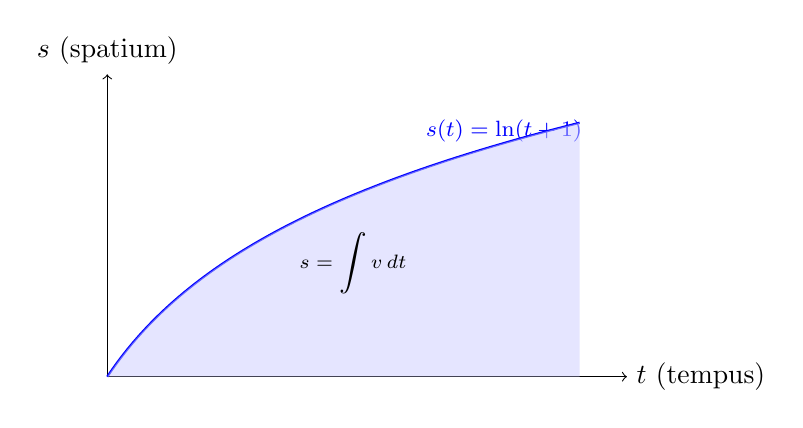
\begin{tikzpicture}[scale=1.2]
  
    % Axes
    \draw[->] (0,0) -- (5.5,0) node[right] {$t$ (tempus)};
    \draw[->] (0,0) -- (0,3.2) node[above] {$s$ (spatium)};
  
    % Curve
    \draw[thick,blue,domain=0:5,smooth,samples=100] plot(\x,{1.5*ln(\x + 1)});
    \node[blue] at (4.2,2.6) {\footnotesize $s(t) = \ln(t + 1)$};
  
    % Fill under curve
    \fill[blue!20,opacity=0.5] (0,0) -- plot[domain=0:5,samples=100] (\x,{1.5*ln(\x + 1)}) -- (5,0) -- cycle;
  
    % Integral label
    \node at (2.6,1.2) {\scriptsize $\displaystyle s = \int v\,dt$};
  
  \end{tikzpicture}
  \caption{The area under the curve $v(t)$ represents accumulated distance. Leibniz expressed this as $s = \int v\,dt$.}
\end{figure}
  

\subsubsection{Integration by Parts: A Rule from Falling Bodies} 

In handling variable motion, Leibniz developed general methods for integrating products of changing quantities. One of these was the rule we now call integration by parts.

He might write it like this:

\[
\int u\,dv = u v - \int v\,du
\]

But for Leibniz, this wasn’t a theorem — it was a technique for transforming one infinitesimal sum into another, more convenient one.

\begin{figure}[H]
\centering
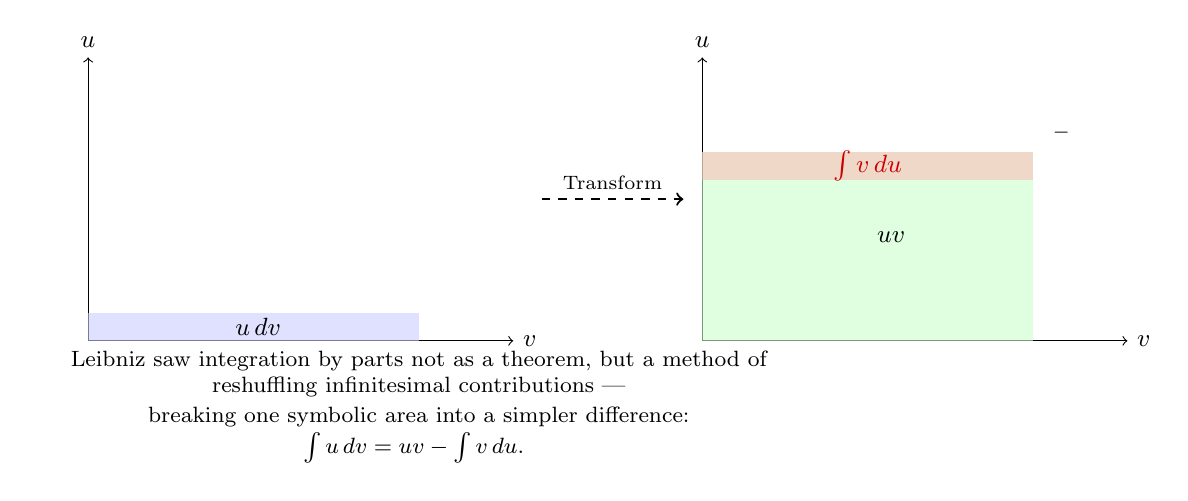
\begin{tikzpicture}[scale=1.2, every node/.style={font=\small}]

  % Axis box for infinitesimal rectangles
  \draw[->] (0,0) -- (4.5,0) node[right] {$v$};
  \draw[->] (0,0) -- (0,3) node[above] {$u$};

  % Rectangle for u dv
  \fill[blue!20,opacity=0.6] (0,0) rectangle (3.5,0.3);
  \node at (1.8,0.15) {$u\,dv$};

  % Dashed arrow to transformed expression
  \draw[->, thick, dashed] (4.8,1.5) -- (6.3,1.5);
  \node[above] at (5.55,1.5) {\scriptsize Transform};

  % Output: uv - ∫v du block
  \begin{scope}[xshift=6.5cm]
    \draw[->] (0,0) -- (4.5,0) node[right] {$v$};
    \draw[->] (0,0) -- (0,3) node[above] {$u$};

    % Highlight uv area (solid block)
    \fill[green!20,opacity=0.6] (0,0) rectangle (3.5,2.0);
    \node at (2.0,1.1) {$uv$};

    % Subtracting integral ∫v du
    \fill[red!30,opacity=0.5] (0,1.7) rectangle (3.5,2.0);
    \node[red!80!black] at (1.75,1.85) {$\int v\,du$};

    % Minus sign
    \node at (3.8,2.2) {\scriptsize $-$};

  \end{scope}

  % Label
  \node at (3.5,-0.7) {
    \begin{minipage}{0.8\linewidth}
      \centering
      {\footnotesize
      Leibniz saw integration by parts not as a theorem, but a method of reshuffling infinitesimal contributions —\\
      breaking one symbolic area into a simpler difference: \quad $\int u\,dv = uv - \int v\,du$.
      }
    \end{minipage}
  };

\end{tikzpicture}
\caption{Leibniz’s idea of integration by parts: transforming one infinitesimal sum into another. Instead of proving a rule, he saw it as a symbolic rearrangement of differentials — from $\int u\,dv$ into $uv - \int v\,du$.}
\end{figure}

\medskip

Kepler’s Second Law tells us that a planet sweeps out \textbf{equal areas in equal times} as it orbits the Sun. Mathematically, this means that the rate of area accumulation, \( \dot{A} \), is constant:

\[
\dot{A} = \frac{1}{2} r^2 \dot{\theta} = \text{constant}
\]

But this constancy masks a deeper complexity in how planets move through space. In particular, while the area swept out increases linearly with time, the \textbf{angular motion} and \textbf{orbital velocity} vary dramatically over the course of the orbit. This nonlinear behavior leads to patterns that, when examined closely, resemble the shape of a logarithmic curve.

\begin{enumerate}
    \item \textbf{Near Perihelion and Aphelion: Logarithmic-like Accumulation}

    A planet moves fastest near perihelion and slowest near aphelion. To maintain a constant area-sweeping rate, its angular velocity \( \dot{\theta} \) must adjust inversely with the square of the radius. This results in angular displacement increasing rapidly at first and then more slowly — an accumulation pattern that echoes logarithmic growth.

    \item \textbf{Time as a Function of Angle}

    In elliptical orbits, time and angular position are not linearly related. Solving Kepler’s equation:

    \[
    M = E - e \sin E
    \]

    requires approximations that include \textbf{transcendental} and even \textbf{logarithmic-like terms}. While area grows uniformly in time, the true anomaly \( \theta(t) \) bends and twists that uniformity into something more intricate.

    \item \textbf{Radial Motion and Logarithmic Divergence}

    In a limiting case where a body falls radially toward the Sun, its velocity increases with decreasing radius. However, the time required to reach the center becomes infinite — a classic case of \textbf{logarithmic divergence}. The motion accelerates, yet never completes in finite time.
\end{enumerate}

\medskip

\noindent These subtle, nonlinear time dependencies lurking beneath Kepler’s geometry provide us with the perfect setting for a symbolic interpretation. Instead of a falling cannonball, we’ll now consider a planet in orbit — moving under the constraint of Kepler’s Second Law — and reinterpret its motion through the lens of Leibniz’s calculus.

\medskip

\noindent In particular, we return to the differential identity:

\[
ds = v\,dt
\]

which tells us that a small displacement \( ds \) is equal to the planet’s velocity multiplied by an infinitesimal duration of time. But what happens if we multiply both sides by \( t \), the elapsed time itself?

\[
t\,ds = t v\,dt
\]

This expression tells us how motion accumulates not just over time, but \textit{weighted} by time — and it sets the stage for an application of \textbf{integration by parts}, which will let us symbolically rearrange and reinterpret the unfolding of planetary motion.



\[
t\,ds = t v\,dt
\]

\begin{figure}[H]
  \centering
  \begin{tikzpicture}[scale=1.2]
  
    % Axes
    \draw[->] (0,0) -- (5.5,0) node[right] {$t$ (tempus)};
    \draw[->] (0,0) -- (0,3.2) node[above] {$s$ (spatium)};
  
    % Curve
    \draw[thick,blue,domain=0:5,smooth,samples=100] plot(\x,{1.5*ln(\x + 1)});
    \node[blue] at (4.2,2.6) {\footnotesize $s(t) = \ln(t + 1)$};
  
    % Point
    \coordinate (P) at (3,{1.5*ln(4)});
    \filldraw[blue] (P) circle (1pt);
    \node[above left] at (P) {\scriptsize $(t, s)$};
  
    % Tangent
    \draw[->, thick,red] (P) -- ++(1, {1.5/(3 + 1)});
    \node[above right] at ($(P)+(1,0.5)$) {\scriptsize $v = \frac{ds}{dt}$};
  
    % Dashed lines
    \draw[dashed] (3,0) -- (P);
    \node[below] at (3,0) {\scriptsize $t$};
    \draw[dashed] (0,{1.5*ln(4)}) -- (3,{1.5*ln(4)});
    \node[left] at (0,{1.5*ln(4)}) {\scriptsize $s$};
  
    % Rectangle
    \fill[blue!20, opacity=0.5] (3,0) rectangle ++(0.3,{1.5/(4)*0.3});
    \node[below right] at (3.1,0.1) {\scriptsize $tv\,dt$};
  
  \end{tikzpicture}
  \caption{Leibniz’s product $tv\,dt$ represents an infinitesimal contribution to position, scaled by time—a key to symbolic mechanics.}
\end{figure}
  


Now consider the integral of the right-hand side:

\[
\int t v\,dt
\]

\begin{figure}[H]
  \centering
  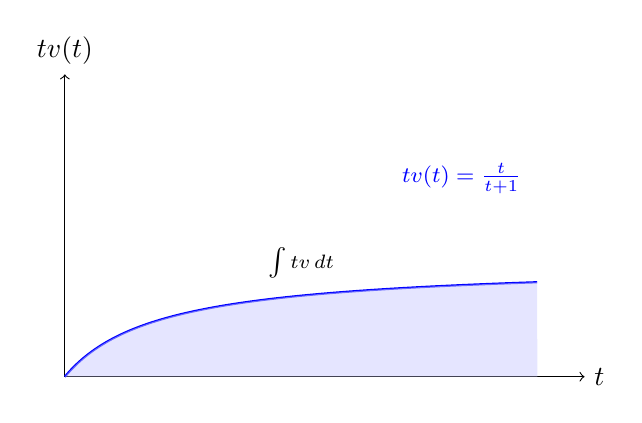
\begin{tikzpicture}[scale=1.2]
  
    % Axes
    \draw[->] (0,0) -- (5.5,0) node[right] {$t$};
    \draw[->] (0,0) -- (0,3.2) node[above] {$tv(t)$};
  
    % Curve: tv = t / (t + 1)
    \draw[thick,blue,domain=0:5,smooth,samples=100] plot(\x,{1.2*\x/(1+\x)});
    \fill[blue!20,opacity=0.5] (0,0) -- plot[domain=0:5,samples=100] (\x,{1.2*\x/(1+\x)}) -- (5,0) -- cycle;
  
    \node[blue] at (4.2,2.1) {\footnotesize $tv(t) = \frac{t}{t + 1}$};
    \node at (2.5,1.2) {\scriptsize $\int tv\,dt$};
  
  \end{tikzpicture}
  \caption{Leibniz’s integration of $tv\,dt$ shows how time-weighted velocity contributes to total motion.}
\end{figure}
  


Let $u = t$, $dv = v\,dt$, so $du = dt$, and $v = s$ (since $ds = v\,dt$). Then, by his rule:

\[
\int t v\,dt = t s - \int s\,dt
\]

\begin{figure}[H]
  \centering
  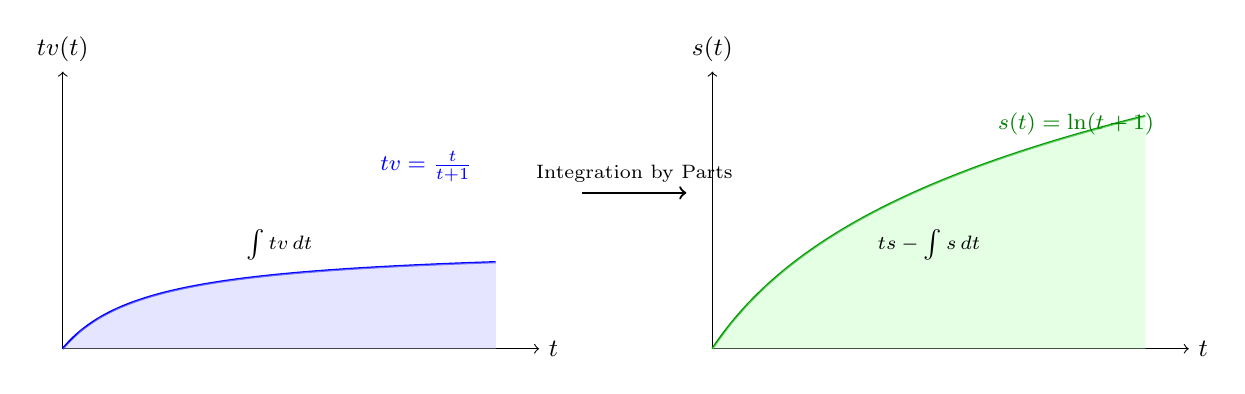
\begin{tikzpicture}[scale=1.1, every node/.style={font=\small}]
  
    % Left side: integral of tv
    \begin{scope}
      \draw[->] (0,0) -- (5.5,0) node[right] {$t$};
      \draw[->] (0,0) -- (0,3.2) node[above] {$tv(t)$};
      \draw[thick,blue,domain=0:5,smooth,samples=100] plot(\x,{1.2*\x/(1+\x)});
      \fill[blue!20,opacity=0.5] (0,0) -- plot[domain=0:5] (\x,{1.2*\x/(1+\x)}) -- (5,0) -- cycle;
      \node[blue] at (4.2,2.1) {\footnotesize $tv = \frac{t}{t+1}$};
      \node at (2.5,1.2) {\scriptsize $\int tv\,dt$};
    \end{scope}
  
    % Arrow
    \draw[->, thick] (6,1.8) -- (7.2,1.8) node[midway, above] {\scriptsize Integration by Parts};
  
    % Right side: ts - ∫s dt
    \begin{scope}[xshift=7.5cm]
      \draw[->] (0,0) -- (5.5,0) node[right] {$t$};
      \draw[->] (0,0) -- (0,3.2) node[above] {$s(t)$};
      \draw[thick,green!60!black,domain=0:5,smooth,samples=100] plot(\x,{1.5*ln(\x + 1)});
      \fill[green!20,opacity=0.5] (0,0) -- plot[domain=0:5] (\x,{1.5*ln(\x + 1)}) -- (5,0) -- cycle;
      \node[green!50!black] at (4.2,2.6) {\footnotesize $s(t) = \ln(t + 1)$};
      \node at (2.5,1.2) {\scriptsize $ts - \int s\,dt$};
    \end{scope}
  
  \end{tikzpicture}
  \caption{Leibniz transformed $\int tv\,dt$ into $ts - \int s\,dt$ — a purely symbolic rearrangement of motion through infinitesimals.}
\end{figure}
  


This gave him a way to understand the accumulation of motion over time in terms of the changing relationship between position and time. Not geometry — but algebraic bookkeeping of motion.

Where Newton used triangles, Leibniz wrote:

\[
dy = f(x)\,dx \quad \Rightarrow \quad y = \int f(x)\,dx
\]

Where Newton argued force from area, Leibniz discovered area from differentials.

\begin{figure}[H]
\centering
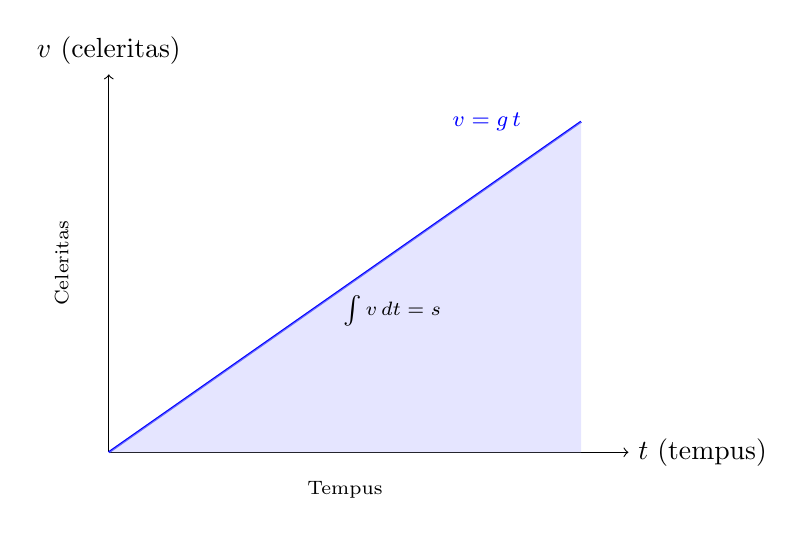
\begin{tikzpicture}[scale=1.2]

  % Axes
  \draw[->] (0,0) -- (5.5,0) node[right] {$t$ (tempus)};
  \draw[->] (0,0) -- (0,4) node[above] {$v$ (celeritas)};

  % Velocity curve: v(t) = g t
  \draw[thick, blue, domain=0:5, samples=100] plot(\x,{0.7*\x});
  \node[blue] at (4,3.5) {\footnotesize $v = g\,t$};

  % Area under curve (shaded)
  \fill[blue!20, opacity=0.5] (0,0) -- plot[domain=0:5] (\x,{0.7*\x}) -- (5,0) -- cycle;

  % Annotations
  \node at (2.5, -0.4) {\scriptsize Tempus};
  \node[rotate=90] at (-0.5, 2) {\scriptsize Celeritas};
  \node at (3,1.5) {\scriptsize $\int v\,dt = s$};

\end{tikzpicture}
\caption{Leibniz’s algebraic conception of motion: the area under the velocity curve represents the distance fallen. Not triangles — but infinitesimals.}
\end{figure}


\begin{tcolorbox}[colback=blue!5!white, colframe=blue!50!black, 
  title={Historical Sidebar: Leibniz—Calculus, Harmony, and the Divine Algorithm}]
  
      \textbf{Gottfried Wilhelm Leibniz} didn’t just co-invent calculus—he invented it as part of a larger metaphysical project: \textbf{to show that the universe was the optimal solution to a divine equation}. For Leibniz, mathematics wasn’t separate from philosophy. It was philosophy, written in symbolic shorthand.
  
      \medskip
  
      His belief in the \textbf{“best of all possible worlds”} had deep theological roots. Leibniz was profoundly influenced by \textbf{Anselm of Canterbury}, the medieval philosopher who defined God as “that than which nothing greater can be conceived.” From that, Leibniz reasoned: if God is maximally perfect and rational, then the world He creates must also reflect that perfection as \textbf{a universe governed by the simplest laws producing the richest variety of outcomes}.
  
      \medskip
  
      This obsession with harmony and optimization laid the philosophical foundation for what would become variational calculus. Leibniz saw nature as a system that doesn’t waste effort—it minimizes and balances, like a cosmic engineer working with divine efficiency.
  
      \medskip
  
      His version of calculus focused on infinitesimals—quantities so small they straddle the line between something and nothing. These weren’t just technical tools. They reflected his belief that \textbf{all change happens gradually, rationally, and with purpose}. Nature, he argued, doesn’t leap; it glides.
  
      \medskip
  
      Even his notation—those now-familiar \texttt{dx} and \texttt{dy} symbols—reflected a vision of the universe as a flowing, continuous, and infinitely divisible system. To Leibniz, calculus was a kind of \textbf{divine syntax}: a universal language that could express not just motion and mechanics, but logic, theology, and metaphysical truth. In short, Leibniz wasn’t just trying to solve math problems. He was trying to read the mind of God... with math.
  
      \medskip
  
      \textbf{Quote from Leibniz (1686):}
      \begin{quote}
      “The present is pregnant with the future; the future could be calculated from it, if we had sufficient knowledge of all causes.”
      \end{quote}
  
  
  \end{tcolorbox}
  







---
